% po4a: environment DndSidebar
% po4a: environment DndTable
\part{Character Creation}
\chapter{Step-by-Step Characters}
\DndDropCapLine{Y}{our first step in playing an adventurer} in the Dungeons \& Dragons game is to imagine and create a character of your own. Your character is a combination of game statistics, roleplaying hooks, and your imagination. You choose a race (such as human or halfling) and a class (such as fighter or wizard). You also invent the personality, appearance, and backstory of your character. Once completed, your character serves as your representative in the game, your avatar in the \textsc{Dungeons \& Dragons} world.

Before you dive into step 1 below, think about the kind of adventurer you want to play. You might be a cou- rageous fighter, a skulking rogue, a fervent cleric, or a flamboyant wizard. Or you might be more interested in an unconventional character, such as a brawny rogue who likes hand-to-hand combat, or a sharpshooter who picks off enemies from afar. Do you like fantasy fiction featuring dwarves or elves? Try building a character of one of those races. Do you want your character to be the toughest adventurer at the table? Consider the fighter class. If you don’t know where else to begin, take a look at the illustrations in this book to see what catches your interest.

Once you have a character in mind, follow these steps in order, making decisions that reflect the character you want. Your conception of your character might evolve with each choice you make. What’s important is that you come to the table with a character you’re excited to play. Throughout this chapter, we use the term \textbf{character sheet} to mean whatever you use to track your character, whether it’s a formal character sheet (like the one at the end of these rules), some form of digital record, or a piece of notebook paper. An official D\&D character sheet is a fine place to start until you know what information you need and how you use it during the game.

\subsubsection{Building Bruenor}
Each step of character creation includes an example of that step, with a player named Bob building his dwarf character, Bruenor.

\subsection{1. Choose a Race}
Every character belongs to a race, one of the many intelligent humanoid species in the D\&D world. The most common player character races are dwarves, elves, halflings, and humans. Some races also have \textbf{subraces}, such as mountain dwarf or wood elf. Chapter 2 provides more information about these races.

The race you choose contributes to your character’s identity in an important way, by establishing a general appearance and the natural talents gained from culture and ancestry. Your character’s race grants particular racial traits, such as special senses, proficiency with certain weapons or tools, proficiency in one or more skills, or the ability to use minor spells. These traits sometimes dovetail with the capabilities of certain classes (see step 2). For example, the racial traits of lightfoot halflings make them exceptional rogues, and high elves tend to be powerful wizards. Sometimes playing against type can be fun, too. Halfling paladins and mountain dwarf wizards, for example, can be unusual but memorable characters.

Your race also increases one or more of your ability scores, which you determine in step 3. Note these in- creases and remember to apply them later.

Record the traits granted by your race on your character sheet. Be sure to note your starting languages and your base speed as well.

\subsubsection{Building Bruenor, Step 1}
Bob is sitting down to create his character. He decides that a gruff mountain dwarf fits the character he wants to play. He notes all the racial traits of dwarves on his character sheet, including his speed of 25 feet and the languages he knows: Common and Dwarvish.

\subsection{2. Choose a Class}
Every adventurer is a member of a class. Class broadly describes a character’s vocation, what special talents he or she possesses, and the tactics he or she is most likely to employ when exploring a dungeon, fighting monsters, or engaging in a tense negotiation. The character classes are described in chapter 3.

Your character receives a number of benefits from your choice of class. Many of these benefits are \textbf{class features}—capabilities (including spellcasting) that set your character apart from members of other classes. You also gain a number of \textbf{proficiencies}: armor, weapons, skills, saving throws, and sometimes tools. Your proficiencies define many of the things your character can do particularly well, from using certain weapons to telling a convincing lie.

On your character sheet, record all the features that your class gives you at 1st level.

\subsubsection{Level}
Typically, a character starts at 1st level and advances in level by adventuring and gaining \textbf{experience points} (XP). A 1st-level character is inexperienced in the adventuring world, although he or she might have been a soldier or a pirate and done dangerous things before.

Starting off at 1st level marks your character’s entry into the adventuring life. If you’re already familiar with the game, or if you are joining an existing D\&D campaign, your DM might decide to have you begin at a higher level, on the assumption that your character has already survived a few harrowing adventures.

Record your level on your character sheet. If you’re starting at a higher level, record the additional elements your class gives you for your levels past 1st. Also record your experience points. A 1st-level character has
0 XP. A higher-level character typically begins with the minimum amount of XP required to reach that level (see “Beyond 1st Level” later in this chapter).

\subsubsection{Hit Points and Hit Dice}
Your character’s hit points define how tough your character is in combat and other dangerous situations. Your hit points are determined by your Hit Dice (short for Hit Point Dice).

At 1st level, your character has 1 Hit Die, and the die type is determined by your class. You start with hit points equal to the highest roll of that die, as indicated in your class description. (You also add your Constitution mod- ifier, which you’ll determine in step 3.) This is also your \textbf{hit point maximum}.

Record your character’s hit points on your character sheet. Also record the type of Hit Die your character uses and the number of Hit Dice you have. After you rest, you can spend Hit Dice to regain hit points (see “Resting” in chapter 8).

\subsubsection{Proficiency Bonus}
The table that appears in your class description shows your proficiency bonus, which is +2 for a 1st-level character. Your proficiency bonus applies to many of the numbers you’ll be recording on your character sheet:

\begin{itemize}
  \item Attack rolls using weapons you’re proficient with
  \item Attack rolls with spells you cast
  \item Ability checks using skills you’re proficient in
  \item Ability checks using tools you’re proficient with
  \item Saving throws you’re proficient in
  \item Saving throw DCs for spells you cast (explained in each spellcasting class)
\end{itemize}

Your class determines your weapon proficiencies, your saving throw proficiencies, and some of your skill and tool proficiencies. (Skills are described in chapter 7, tools in chapter 5.) Your background gives you additional skill and tool proficiencies, and some races give you more proficiencies. Be sure to note all of these proficiencies, as well as your proficiency bonus, on your character sheet.

Your proficiency bonus can’t be added to a single die roll or other number more than once. Occasionally, your proficiency bonus might be modified (doubled or halved, for example) before you apply it. If a circumstance sug- gests that your proficiency bonus applies more than once to the same roll or that it should be multiplied more than once, you nevertheless add it only once, multiply it only once, and halve it only once.

\subsubsection{Building Bruenor, Step 2}
Bob imagines Bruenor charging into battle with an axe, one horn on his helmet broken off. He makes Bruenor a fighter and notes the fighter’s proficiencies and 1st-level class features on his character sheet.

As a 1st-level fighter, Bruenor has 1 Hit Die—a d10— and starts with hit points equal to 10 + his Constitution modifier. Bob notes this, and will record the final number after he determines Bruenor’s Constitution score (see step 3). Bob also notes the proficiency bonus for a 1st- level character, which is +2.

\begingroup
  \DndSetThemeColor[PhbTan]
  \begin{DndSidebar}{Quick Build}
    Each class description in chapter 3 includes a section offering suggestions to quickly build a character of that class, including how to assign your highest ability scores, a background suitable to the class, and starting spells.
  \end{DndSidebar}
\endgroup

\subsection{3. Determine Ability Scores}
Much of what your character does in the game depends on his or her six abilities: \textbf{Strength}, \textbf{Dexterity}, \textbf{Constitution}, \textbf{Intelligence}, \textbf{Wisdom}, and \textbf{Charisma}. Each ability has a score, which is a number you record on your character sheet.

The six abilities and their use in the game are de- scribed in chapter 7. The Ability Score Summary table provides a quick reference for what qualities are measured by each ability, what races increases which abilities, and what classes consider each ability particu- larly important.

You generate your character’s six ability scores randomly. Roll four 6-sided dice and record the total of the highest three dice on a piece of scratch paper. Do this five more times, so that you have six numbers. If you want to save time or don’t like the idea of randomly determining ability scores, you can use the following scores instead: 15, 14, 13, 12, 10, 8.

Now take your six numbers and write each number beside one of your character’s six abilities to assign scores to Strength, Dexterity, Constitution, Intelligence, Wisdom, and Charisma. Afterward, make any changes to your ability scores as a result of your race choice.

After assigning your ability scores, determine your \textbf{ability modifiers} using the Ability Scores and Modifiers table. To determine an ability modifier without consulting the table, subtract 10 from the ability score and then divide the result by 2 (round down). Write the modifier next to each of your scores.

\subsubsection{Building Bruenor, Step 3}
Bob decides to use the standard set of scores (15, 14, 13, 12, 10, 8) for Bruenor’s abilities. Since he’s a fighter, he puts his highest score, 15, in Strength. His next-highest, 14, goes in Constitution. Bruenor might be a brash fighter, but Bob decides he wants the dwarf to be older, wiser, and a good leader, so he puts decent scores in Wisdom and Charisma. After applying his racial ben- efits (increasing Bruenor’s Constitution by 2 and his Strength by 2), Bruenor’s ability scores and modifiers look like this: Strength 17 (+3), Dexterity 10 (+0), Constitution 16 (+3), Intelligence 8 (–1), Wisdom 13 (+1), Charisma 12 (+1).

Bob fills in Bruenor’s final hit points: 10 + his Constitution modifier of +3, for a total of 13 hit points.

\begingroup
  \DndSetThemeColor[PhbTan]
  \begin{table}[!htb]
    \caption{\DndFontTableTitle{}Ability Scores and Modifiers}
    \begin{minipage}{.5\linewidth}
        \begin{DndTable}{cc}
          Score & Modifier \\
          1     & -5       \\
          2–3   & -4       \\
          4-5   & -3       \\
          6-7   & -2       \\
          8-9   & -1       \\
          10-11 & +0       \\
          12-13 & +1       \\
          14-15 & +2       \\
        \end{DndTable}
    \end{minipage}%
    \begin{minipage}{.5\linewidth}
        \begin{DndTable}{cc}
          Score & Modifier \\
          16-17 & +3       \\
          18-19 & +4       \\
          20-21 & +5       \\
          22-23 & +6       \\
          24-25 & +7       \\
          26-27 & +8       \\
          28-29 & +9       \\
          30    & +10      \\
        \end{DndTable}
    \end{minipage} 
  \end{table}
\endgroup

\begin{DndTable}[header=Ability Score Summary]{X}
  \rowcolor{PhbTan} \textbf{Strength} \\
  \hiderowcolors \textit{Measures: Natural athleticism, bodily power \newline
    Important for: Fighter \newline
    Racial Increases: \newline
    \ \ \ Mountain dwarf (+2) \newline
    \ \ \ Human (+1)
    \newline } \\
  \rowcolor{PhbTan} \textbf{Dexterity} \\
  \hiderowcolors \textit{Measures: Physical agility, reflexes, balance, poise \newline
    Important for: Rogue \newline
    Racial Increases: \newline
    \ \ \ Elf (+2)\tab Human (+1) \newline
    \ \ \ Halfling (+2) \newline
    \newline } \\
  \rowcolor{PhbTan} \textbf{Constitution} \\
  \hiderowcolors \textit{Measures: Health, stamina, vital force \newline
    Important for: Everyone \newline
    Racial Increases: \newline
    \ \ \ Dwarf (+2) \newline
    \ \ \ Stout halfling (+1) \newline
    \ \ \ Human (+1) \newline
    \newline } \\
  \rowcolor{PhbTan} \textbf{Intelligence} \\
  \hiderowcolors \textit{Measures: Mental acuity, information recall, analytical skill \newline
    Important for: Wizard \newline
    Racial Increases: \newline
    \ \ \ High elf (+1) \newline
    \ \ \ Human (+1)
    \newline } \\
  \rowcolor{PhbTan} \textbf{Wisdom} \\
  \hiderowcolors \textit{Measures: Awareness, intuition, insight \newline
    Important for: Cleric \newline
    Racial Increases: \newline
    \ \ \ Hill dwarf (+1)\tab Human (+1) \newline
    \ \ \ Wood elf (+1)
    \newline } \\
  \rowcolor{PhbTan} \textbf{Charisma} \\
  \hiderowcolors \textit{Measures: Confidence, eloquence, leadership \newline
    Important for: Leaders and diplomatic characters \newline
    Racial Increases: \newline
    \ \ \ Lightfoot halfling (+1)\tab Human (+1) \newline
    \newline }
\end{DndTable}

\subsubsection{Variant: Customizing Ability Scores}
At your Dungeon Master’s option, you can use this variant for determining your ability scores. The method described here allows you to build a character with a set of ability scores you choose individually.

You have 27 points to spend on your ability scores. The cost of each score is shown on the Ability Score Point Cost table. For example, a score of 14 costs 7 points. Using this method, 15 is the highest ability score you can end up with, before applying racial increases. You can’t have a score lower than 8.

This method of determining ability scores enables you to create a set of three high numbers and three low ones (15, 15, 15, 8, 8, 8), a set of numbers that are above average and nearly equal (13, 13, 13, 12, 12, 12), or any set of numbers between those extremes.

\begingroup
  \DndSetThemeColor[PhbTan]
  \begin{table}[!htb]
    \caption{\DndFontTableTitle{}Ability Score Point Cost}
    \begin{minipage}{.5\linewidth}
        \begin{DndTable}{cc}
          Score & Cost     \\
          8     & 0        \\
          9     & 1        \\
          10    & 2        \\
          11   & 3         \\
        \end{DndTable}
    \end{minipage}%
    \begin{minipage}{.5\linewidth}
        \begin{DndTable}{cc}
          Score & Cost     \\
          12    & 4        \\
          13    & 5        \\
          14    & 7        \\
          15    & 9        \\
        \end{DndTable}
    \end{minipage} 
  \end{table}
\endgroup

\subsection{4. Describe Your Character}
Once you know the basic game aspects of your character, it’s time to flesh him or her out as a person. Your character needs a name. Spend a few minutes thinking about what he or she looks like and how he or she behaves in general terms.

Using the information in chapter 4, you can flesh out your character’s physical appearance and personality traits. Choose your character’s \textbf{alignment} (the moral compass that guides his or her decisions) and \textbf{ideals}. Chapter 4 also helps you identify the things your character holds most dear, called \textbf{bonds}, and the \textbf{flaws} that could one day undermine him or her.

Your character’s \textbf{background} describes where he or she came from, his or her original occupation, and the character’s place in the D\&D world. Your DM might offer additional backgrounds beyond the ones included in chapter 4, and might be willing to work with you to craft a background that’s a more precise fit for your character concept.

A background gives your character a background feature (a general benefit) and proficiency in two skills, and it might also give you additional languages or proficiency with certain kinds of tools. Record this information, along with the personality information you develop, on your character sheet.

\subsubsection{Your Character’s Abilities}
Take your character’s ability scores and race into account as you flesh out his or her appearance and personality. A very strong character with low Intelligence might think and behave very differently from a very smart character with low Strength.

For example, high Strength usually corresponds with a burly or athletic body, while a character with low Strength might be scrawny or plump.

A character with high Dexterity is probably lithe and slim, while a character with low Dexterity might be either gangly and awkward or heavy and thick-fingered.

A character with high Constitution usually looks healthy, with bright eyes and abundant energy. A character with low Constitution might be sickly or frail.

A character with high Intelligence might be highly inquisitive and studious, while a character with low Intelligence might speak simply or easily forget details.

A character with high Wisdom has good judgment, em- pathy, and a general awareness of what’s going on. A character with low Wisdom might be absent-minded, foolhardy, or oblivious.

A character with high Charisma exudes confidence, which is usually mixed with a graceful or intimidating presence. A character with a low Charisma might come across as abrasive, inarticulate, or timid.

\subsubsection{Building Bruenor, Step 4}
Bob fills in some of Bruenor’s basic details: his name, his sex (male), his height and weight, and his alignment (lawful good). His high Strength and Constitution suggest a healthy, athletic body, and his low Intelligence suggests a degree of forgetfulness.

Bob decides that Bruenor comes from a noble line, but his clan was expelled from its homeland when Bruenor was very young. He grew up working as a smith in the remote villages of Icewind Dale. But Bruenor has a heroic destiny—to reclaim his homeland—so Bob chooses the folk hero background for his dwarf. He notes the proficiencies and special feature this background gives him.

Bob has a pretty clear picture of Bruenor’s personality in mind, so he skips the personality traits suggested in the folk hero background, noting instead that Bruenor is a caring, sensitive dwarf who genuinely loves his friends and allies, but he hides this soft heart behind a gruff, snarling demeanor. He chooses the ideal of fairness from the list in his background, noting that Bruenor believes that no one is above the law.

Given his history, Bruenor’s bond is obvious: he aspires to someday reclaim Mithral Hall, his homeland, from the shadow dragon that drove the dwarves out. His flaw is tied to his caring, sensitive nature—he has a soft spot for orphans and wayward souls, leading him to show mercy even when it might not be warranted.

\subsection{5. Choose Equipment}
Your class and background determine your character’s \textbf{starting equipment}, including weapons, armor, and other adventuring gear. Record this equipment on your character sheet. All such items are detailed in chapter 5, “Equipment.“

Instead of taking the gear given to you by your class and background, you can purchase your starting equipment. You have a number of \textbf{gold pieces} (gp) to spend based on your class, as shown in chapter 5. Extensive lists of equipment, with prices, also appear in that chap- ter. If you wish, you can also have one trinket at no cost (see the Trinkets table at the end of chapter 5).
Your Strength score limits the amount of gear you can carry. Try not to purchase equipment with a total weight (in pounds) exceeding your Strength score times 15. Chapter 7 has more information on carrying capacity.

\subsubsection{Armor Class}
Your \textbf{Armor Class} (AC) represents how well your character avoids being wounded in battle. Things that contribute to your AC include the armor you wear, the shield you carry, and your Dexterity modifier. Not all characters wear armor or carry shields, however.

Without armor or a shield, your character’s AC equals 10 + his or her Dexterity modifier. If your character wears armor, carries a shield, or both, calculate your AC using the rules in chapter 5. Record your AC on your character sheet.

Your character needs to be proficient with armor and shields to wear and use them effectively, and your armor and shield proficiencies are determined by your class. There are drawbacks to wearing armor or carrying a shield if you lack the required proficiency, as explained in chapter 5.

Some spells and class features give you a different way to calculate your AC. If you have multiple features that give you different ways to calculate your AC, you choose which one to use.

\subsubsection{Weapons}
For each weapon your character wields, calculate the modifier you use when you attack with the weapon and the damage you deal when you hit.

When you make an attack with a weapon, you roll a d20 and add your proficiency bonus (but only if you are proficient with the weapon) and the appropriate ability modifier.

\begin{itemize}
  \item For attacks with \textbf{melee weapons}, use your Strength modifier for attack and damage rolls. A weapon that has the finesse property, such as a rapier, can use your Dexterity modifier instead.
  \item For attacks with \textbf{ranged weapons}, use your Dexterity modifier for attack and damage rolls. A melee weapon that has the thrown property, such as a handaxe, can use your Strength modifier instead.
\end{itemize}

\subsubsection{Building Bruenor, Step 5}
Bob writes down the starting equipment from the fighter class and the folk hero background. His starting equipment includes chain mail and a shield, which combine to give Bruenor an Armor Class of 18.

For Bruenor’s weapons, Bob chooses a battleaxe and two handaxes. His battleaxe is a melee weapon, so Bruenor uses his Strength modifier for his attacks and damage. His attack bonus is his Strength modifier (+3) plus his proficiency bonus (+2), for a total of +5. The bat- tleaxe deals 1d8 slashing damage, and Bruenor adds his Strength modifier to the damage when he hits, for a total of 1d8 + 3 slashing damage. When throwing a handaxe, Bruenor has the same attack bonus (handaxes, as thrown weapons, use Strength for attacks and damage), and the weapon deals 1d6 + 3 slashing damage when it hits.

\subsection{6. Come Together}
Most D\&D characters don’t work alone. Each character plays a role within a \textbf{party}, a group of adventurers working together for a common purpose. Teamwork and cooperation greatly improve your party’s chances to survive the many perils in the worlds of Dungeons \& Dragons. Talk to your fellow players and your DM to decide whether your characters know one another, how they met, and what sorts of quests the group might undertake.

\section{Beyond 1st Level}
As your character goes on adventures and overcomes challenges, he or she gains experience, represented by experience points. A character who reaches a specified experience point total advances in capability. This ad- vancement is called \textbf{gaining a level}.

When your character gains a level, his or her class often grants additional features, as detailed in the class description. Some of these features allow you to increase your ability scores, either increasing two scores by 1 each or increasing one score by 2. You can’t increase an ability score above 20. In addition, every character’s proficiency bonus increases at certain levels.

Each time you gain a level, you gain 1 additional Hit Die. Roll that Hit Die, add your Constitution modifier to the roll, and add the total (minimum of 1) to your hit point maximum. Alternatively, you can use the fixed value shown in your class entry, which is the average result of the die roll (rounded up).

When your Constitution modifier increases by 1, your hit point maximum increases by 1 for each level you have attained. For example, when Bruenor reaches 8th level as a fighter, he increases his Constitution score from 17 to 18, thus increasing his Constitution modifier from +3 to +4. His hit point maximum then increases by 8.

The Character Advancement table summarizes the XP you need to advance in levels from level 1 through level 20, and the proficiency bonus for a character of that level. Consult the information in your character’s class description to see what other improvements you gain at each level.

\subsection{Tiers of Play}
The shading in the Character Advancement table shows the four tiers of play. The tiers don’t have any rules associated with them; they are a general description of how the play experience changes as characters gain levels.
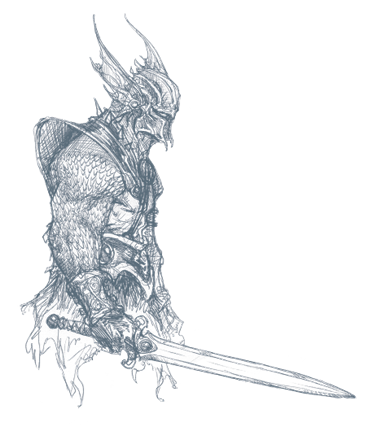
\includegraphics{img/char01.png}

In the first tier (levels 1–4), characters are effectively apprentice adventurers. They are learning the features that define them as members of particular classes, including the major choices that flavor their class features as they advance (such as a wizard’s Arcane Tradition or a fighter’s Martial Archetype). The threats they face are relatively minor, usually posing a danger to local farmsteads or villages.

In the second tier (levels 5–10), characters come into their own. Many spellcasters gain access to 3rd-level spells at the start of this tier, crossing a new threshold of magical power with spells such as fireball and lightning bolt. At this tier, many weapon-using classes gain the ability to make multiple attacks in one round. These characters have become important, facing dangers that threaten cities and kingdoms.

In the third tier (levels 11–16), characters have reached a level of power that sets them high above the ordinary populace and makes them special even among adventurers. At 11th level, many spellcasters gain access to 6th-level spells, some of which create effects previously impossible for player characters to achieve. Other charac- ters gain features that allow them to make more attacks or do more impressive things with those attacks. These mighty adventurers often confront threats to whole regions and continents.

At the fourth tier (levels 17–20), characters achieve the pinnacle of their class features, becoming heroic (or villainous) archetypes in their own right. The fate of the world or even the fundamental order of the multiverse might hang in the balance during their adventures.

\begin{DndTable}[color=PhbTan, header=Character Advancement]{ X c c }
  Experience Points & Level & Proficiency Bonus \\
  0 & 1 & +2 \\
  \rowcolor{PhbTan} 300 & 2 & +2 \\
  \rowcolor{PhbTan} 900 & 3 & +2 \\
  \rowcolor{PhbTan} 2,700 & 4 & +2 \\
  \hiderowcolors 6,500 & 5 & +3 \\
  \hiderowcolors 14,000 & 6 & +3 \\
  \hiderowcolors 23,000 & 7 & +3 \\
  \hiderowcolors 34,000 & 8 & +3 \\
  \rowcolor{PhbTan} 85,000 & 11 & +4 \\
  \rowcolor{PhbTan} 100,000 & 12 & +4 \\
  \rowcolor{PhbTan} 120,000 & 13 & +5 \\
  \rowcolor{PhbTan} 140,000 & 14 & +5 \\
  \rowcolor{PhbTan} 165,000 & 15 & +5 \\
  \rowcolor{PhbTan} 195,000 & 16 & +5 \\
  \hiderowcolors 225,000 & 17 & +6 \\
  \hiderowcolors 265,000 & 18 & +6 \\
  \hiderowcolors 305,000 & 19 & +6 \\
  \hiderowcolors 355,000 & 20 & +6 \\
\end{DndTable}